\documentclass[1p]{elsarticle}

\usepackage{amssymb,amsmath}
\usepackage{graphicx} 

\journal{Journal of Parallel and Distributed Computing}

\begin{document}
\begin{frontmatter}

\title{GPU Accelerated Particle Visualization with Splotch}
\author[1]{Marzia Rivi} 
\address[1]{Department of Physics, University of Oxford, Keble Road, OX1 3RH Oxford, United Kingdom}
\author[2]{Claudio Gheller}
\address[2]{ETH-CSCS, via Trevano 131, 6900 Lugano, Switzerland}
\author[3]{Mel Krokos}
\address[3]{...  University of Portsmouth, ...}
\author[4]{Klaus Dolag}
\address[4]{}
\author[5]{Martin Reinecke}
\address[5]{}

\begin{abstract}
Splotch is a light and fast software tool for visualization of point-like datasets, coming from astronomical observations or numerical particle-based computer simulations. Its main peculiarities are represented by high quality images, obtained by adopting a specialized ray-tracing approach, and the support of large data volumes by the exploitation of multi-core and multi-node systems by means of an effective mix of the OpenMP and MPI parallel programming paradigms. In order to exploit GPUs as well, a CUDA version of Splotch has been implemented. The main steps required to adapt the Splotch algorithm to GPU architectures and get good performances out of it are described. Results of a number of tests and benchmarks are also presented. 
\end{abstract}

\begin{keyword}
Scientific visualization \sep GPU \sep CUDA
\end{keyword}

\end{frontmatter}

\section{Introduction}
\label{sec:intro}

%CLAUDIO: I REMOVED ALL THE REFERENCES HERE SINCE THE SUBJECT IS TOO GENERIC AND BROAD. WE SHOULD CITE HUNDREDS OF PAPER.
The management and analysis of modern, large-scale datasets generated by scientific experiments and numerical simulations, can be very challenging due to continuously increasing sizes and complexity. Traditional data mining and analysis methods often rely on computationally complex
algorithms which can be very expensive if employed for 
large-scale datasets. Visual exploration and discovery can then represent invaluable tools, e.g. by providing scientists with prompt and intuitive insights enabling them to identify interesting characteristics and thus define regions of interest within which
to apply time-consuming methods. Additionally, they can be a very effective way in discovering and understanding correlations in data patterns, or in identifying unexpected behaviours, thus saving valuable resources, e.g. by terminating promptly on going numerical simulations producing unreliable results. Visual exploration and discovery tools can also provide effective means for communicating scientific results not only to researchers but also to members of the general public.

Astrophysics represents a prime example of a scientific field where visual data analysis and exploration is not just useful, but, in some cases, mandatory. Often, in fact, no automated software based solution exists to identify and judge features that requires the human assessment to be correctly interpreted. For this reason, the astrophysical community has a long tradition in developing and deploying visual discovery tools for large-scale datasets represented by images, complex surveys, data cubes or N-body simulations. Consequently astrophysics represents an ideal discipline for exploiting High Performance Computing (HPC) devices, e.g. large multi-core and multi-node systems, providing all necessary resources for coping with large-scale datasets, e.g. computational power, large memory sizes, sufficient storage capacities and fast network speeds. A recent example is given by Hassan et al. (see related works and references in~\cite{2012ASPC..461...45H}), who focus on forthcoming generations of radio surveys (ASKAP~\cite{askap} and SKA~\cite{ska}), which are expected to produce very large datasets. Visual tools play a crucial role in exploring data cubes through a mesh-based volume rendering approach boosted by the efficient usage of GPUs. A further example, is given by Fraedrich et al. \cite{Fraedrich:2009:TMV}, who
investigated scalability in visualizing large-scale particle-based cosmological 
simulations focusing on the Millennium run \cite{millennium}, and presented methods to reduce the associated limitations on PC architectures based on levels-of-detail.
Recently Kaheler et al. \cite{2012arXiv1208.3206K} presented an algorithm specifically designed for N-body simulations. Their approach is based on a tetrahedral tessellation of the computational domain with mesh vertices defined by the simulation's dark matter particle positions and offers several GPU-assisted rendering solutions. This article includes an excellent review of methods for effective visualisation of particle based datasets (the reader is referred to \cite{2012arXiv1208.3206K} for details).

A number of popular, open-source software packages attempt to address the challenges associated with large-scale datasets and exploitation of HPC devices, e.g. VisIt~\cite{visit} and Paraview~\cite{paraview}. Both are based on VTK~\cite{vtk} and support a fairly large variety of data types, file formats and visual discovery solutions. They can be used either as stand alone tools (running on a user's workstation) or in a client-server configuration (deploying services remotely). Both tools support in-situ visualization~\cite{in-situ} allowing visualization procedures to be embedded in a simulation, thus generating images during a run (i.e. no data files are required) and enabling computational steering. A recent application of ParaView to large-scale cosmological simulations can be found in \cite{2011ApJS..195...11W}. Neither of these packages provides customised tools for astrophysics,  e.g. particle visualization capabilities are limited. Often the underlying computational performances and/or memory usage are not highly optimized, thus preventing effective deployment of these packages on modern, large-scale astrophysical datasets. A VTK-based open-source software package focusing on astrophysics is VisIVO~\cite{visivo}. Although its main limitation is lack of interactivity, it has been recently released in the form of a science gateway offering a web-based, workflow-enabled framework seamlessly integrating large-scale, multi-dimensional datasets and applications for processing and visualization by exploiting distributed computing infrastructures \cite{VisIVOGateway}. Advanced users are able to create, change, invoke, and monitor workflows while standard users are provided with customized web interfaces hiding all underlying technical aspects. Tipsy \cite{tipsyurl} and Splash \cite{splash} are further examples of software packages specifically designed for particle-based datasets. Applicability of these packages to large-scale datasets is limited as they operate in stand-alone mode without any support for HPC resources.

This paper concentrates on {\it Splotch} \cite{2008NJPh...10l5006D} which is a ray-casting algorithm for effectively visualizing large-scale, particle-based numerical simulations. Very high-quality visualisations can be generated by Splotch for modern large-scale cosmological simulations, e.g. the Millennium trilogy \cite{millennium}, the Horizon and MareNostrum runs \cite{horizon} or the DEUS simulation \cite{deus}. The underlying models in these simulations typically reproduce the evolution of a representative fraction of the universe by means of hundreds of billions of fluid elements (represented as particles), interacting through gravitational forces. The typical size of a time output (or {\it snapshot}) employed by Splotch can range from several hundreds of GigaBytes (GBs) to tens of TeraBytes (TBs), recording ID, position and velocity of particles together with additional properties, e.g. local smoothing length, density and velocity dispersion. Although developed for numerical simulations, Splotch has being successfully used 
also in other contexts, e.g. visualizing real galaxy systems \cite{m83-vis}.

%, whose 3D shape is carefully modeled
%according to observational data. Here, more than the data size, the driver is
%the quality and the level of details of the final images,
%that have to reproduce the full details and the
%spectacular features of astronomical objects. Furthermore,
%it was adopted also for the visualization of meshed based astrophysical simulations
%(although the same high quality cannot be achieved unless extremely high resolution
%meshes are provided).

The original Splotch algorithm has been optimized in terms of memory usage and exploitation of standard HPC architectures, e.g. multi-core processors and multi-node supercomputing systems by adopting the MPI paradigm \cite{jin:high-performance} and OpenMP (see Section~2). However nowadays HPC systems are increasingly populated with GPUs employed not just as graphic accelerators but also as computational co-processors providing, on suitable classes of algorithms, outstanding performances with power consumption being comparable to standard CPUs. Supercomputers are thus increasingly equipped with several hundreds of GPUs that can overlap their computing capability with that of CPUs, minimising considerably overall times-to-solution of high-end scientific problems.

This paper discusses the issues we faced in designing and implementing a new version of Splotch using the CUDA paradigm to fully exploit modern HPC infrastructures. The main issue was optimizing rendering of variable radius particles, dependent both on their intrinsic size and on the point of view, posing several problems for the GPU computation in terms of race conditions and workload balancing. A preliminary investigation, reported in \cite{jin:high-performance}, had to be redesigned from the ground up to significantly improve the performance. A number of optimized solutions for rendering particles have been implemented, based on a novel data classification and organization strategy. Furthermore, the Thrust library \cite{thrusturl} was adopted for an optimal implementation of specific kernels requiring sorting or reduce-by-key operations.
%CLAUDIO: I WOULD NOT PUT THIS HERE
%Our approach can accelerate the original Splotch up to a factor of 6, when compared to a single core, and 
%can give performance comparable to that of 8 cores using the shared memory parallel model. 
This improved performance is achieved without affecting the performance features of the original Splotch - linear scalability on the number of particles. 
Section~2 is a short description of the Splotch algorithmic approach. Background on CUDA paradigm and a performance model that guided our re-designing of Splotch are discussed in Section~3. Our implementation is presented in Section~4 in which we describe our strategy on how to classify particles and rendering them accordingly. Section~5 presents our reference datasets for benchmarking and discusses performance results including scalability related to sizes of datasets and smoothing radius. Section~6 presents conclusions and pointers to future developments.

\section{Splotch Overview}
\label{sec:overview}

Splotch generates high-quality images through a customised ray-casting approach, described in detail in \cite{2008NJPh...10l5006D}.  
The implementation of Splotch is self-contained with no dependencies from external libraries (apart of course from those needed for parallelism and to support specific file formats, e.g. HDF5 \cite{hdf5}). The code is pure C++ and compilation is straightforward through suitable makefile scripts.
%The current implementation of Splotch \cite{} adheres to a simple software engineering design allowing for easy extensions, e.g. incorporating new data readers. 
To aid the presentation in this paper the main stages of Splotch are summarised as below:
\begin{itemize}
\item
{\it Data Loading} - Several readers are available supporting different formats. As a minimum, three scalars are required, representing particles' cartesian coordinates in a generic phase space (usually geometric coordinates are used but any other meaningful choice is possible).
\item
{\it Processing and Rasterization} - Normalisation together with other necessary 
calculations (e.g. logarithms of processed quantities) are performed. Particle
coordinates and other geometric quantities (e.g. smoothing lengths - see below) are
roto-translated and projected according to camera settings.
Active particles (i.e. contributing to the final rendering) are identified and RGB color components are assigned to each of them.
For the sake of simplicity in the following sections 
this phase will be referred to as {\it Rasterization}.
\item
{\it Rendering} - The contributions of individual particles to pixels of the final 
image are calculated by solving the radiative transfer equation  \cite{1991par..book.....S} along a line of sight originating from each pixel:
\begin{equation}\label{rad}
\frac{d{\bf I}{(\bf x})}{dx}=({\bf E}_p-{\bf A}_p{\bf I}({\bf x}))\rho_p({\bf x}),
\end{equation}
where ${\bf I}({\bf x})$ represents the radiation intensity at position ${\bf x}$, $x$ is is the coordinate along the optical path,  ${\bf E}_p$ and ${\bf A}_p$ are the coefficients of radiation emission and absorption of particle $p$ respectively, and $\rho_p({\bf x})$ is the physical quantity (e.g. mass density or temperature) transported by the particle $p$, with coordinates ${\bf x}_p$, according to a Gaussian distribution:
\begin{equation}\label{kernel}
\rho_p({\bf x}) = \rho_{0,p}\exp(-{||{\bf x}-{\bf x}_p||}^2/\sigma_p^2).
\end{equation}
 
%begin{equation}\label{smooth}
%\rho({\bf x}) = \sum_{p=1}^{N_{part}} \rho_p W(r_p,\sigma_p,\chi),
%\end{equation}
%where $\rho_p$ is a discrete field transported by particles (e.g. mass density or temperature), and $W(r_p,\sigma_p,\chi)$ is a smoothing kernel defined as:
%\begin{equation}\label{kernel}
%W(r_p,\sigma_p,\chi) = \exp(-r_p^2/\sigma_p^2)\qquad {\rm for}\quad  r<\chi\sigma_p,
%\end{equation}
%and
%\begin{equation}\label{kernel1}
%W(r_p,\sigma_p,\chi) = 0 \qquad {\rm for}\quad r>\chi\sigma_p,
%\end{equation}
%where
%$r=\vert {\bf x_p}-{\bf x} \vert$ is the distance of the particle $p$ with coordinates ${\bf x_p}$ from ${\bf x}$ and $\sigma_p$ is a smoothing length defining a compact support for the Gaussian distribution. 
The distribution is considered to be zero at a given distance $\chi\cdot\sigma_p$, 
where $\chi$ is a suitably-defined multiplicative factor and $\sigma_p$ is the particle smoothing length, 
so that any rays passing at 
distances larger than $\chi\sigma_p$ are completely unaffected by $\rho_p$.

In general it is recommended to set ${\bf E}_p = {\bf A}_p$,
which typically produces visually appealing images.
This makes the calculation independent of integration order of particles, allowing a simplified parallel implementations of the algorithm.
For special applications,
independent emission and absorption coefficients can be used. These coefficients
can vary between particles, and are typically chosen as a function of a characteristic
particle property (e.g. its temperature, density, etc.).

%For most of astrophysical applications, where matter density is usually extremely low, the equation can be solved in the {\it optically thin} regime, where the absorption and emission terms are independent of particles. 
%can be neglected. 
%This makes the calculation independent of integration order of particles, allowing a simplified parallel implementations of the algorithm, without affecting the rendering quality and the correctedness of the images. 

Equation \eqref{rad} is solved for each color component (R, G and B). Such components can be defined by exploiting different physical quantities. For instance, colors  can be associated to the three components of the velocity field $\bf v$, so that 
$\rho_p^{R}=v_x$, $\rho_p^{G}=v_y$ and $\rho_p^{B}=v_z$. Conversely, a scalar quantity, such as mass density or temperatures, can be mapped to the RGB components via color look-up tables (or palettes). 
\end{itemize}
Large-scale datasets are supported by exploiting HPC architectures by means of an effective mix of OpenMP / MPI parallel programming paradigms. The MPI implementation~\cite{jin:high-performance}  simply distributes chunks of particles among several tasks, each one performing a serial computation and producing a partial image. The final image is finally composed by the root processor.  
 
The OpenMP implementation splits the {\it Rasterization} loops on particles among several threads. While, for the {\it Rendering} stage the full image is subdivided into tiles of $100 \times 100$ pixels (size can be changed easily) which are processed by the OpenMP threads on a "first-come, first-serve" basis. To determine which subset of particles needs to be considered for a given tile, the whole particle array is scanned before the actual rendering step, and for each tile a list is created, which contains all particle indices that affect the tile. This step is implemented in an OpenMP-parallel fashion as well.

%\begin{figure}
%\centering
%\includegraphics[scale=0.18]{images/flowsplotch.eps}
%\caption{Splotch workflow}
%\label{fig:workflow}
%\end{figure}

\section{GPU Considerations}
\label{sec:gpu-code}

Splotch has been enabled to GPU by exploiting the CUDA programming model. In this section, we review the fundamentals of CUDA programming and introduce the details of a performance model developed to guide the accomplished refactoring work.  

\subsection{CUDA Paradigm} 
\label{sec:cuda}

The CUDA programming model \cite{cudaurl} by NVIDIA currently represents the standard ``de facto'' for GPU programming. The underlying GPUs are closely mapped leading to optimal performances. The obvious drawback of limited portability is somewhat mitigated by the diffusion of NVIDIA GPUs. Access to highly parallelized modern GPU architectures is offered through a simplified C/C++ or Fortran API supporting joint CPU/GPU execution. Serial procedures are performed by the CPU (host), while those which exhibit rich amount of data parallelism are performed by the GPU (device) realized as CUDA kernels. The CPU and GPU have their own memory spaces so data transfers from each other must use the PCI Express bus (hereafter PCI-E). 

The launch of CUDA kernels is asynchronous allowing the host to execute code instructions while the device is computing. If the host requires a kernel execution to be completed then it is necessary to call a device synchronization function. A kernel is instantiated as a grid of lightweight parallel threads organized into blocks of the same size. A thread represents an independent work element and maps to a hardware core (or streaming processor - SP). A {\em block} is a 1D, 2D or 3D set of concurrently executing threads that can cooperate among themselves via barrier synchronization and fast shared memory. This is possible because threads belonging to the same block are executed on the same streaming multiprocessor - SM. However synchronization is not possible between blocks. The limited amount of memory limits the number of  blocks that can reside in a particular SM simultaneously. Moreover when the execution of a block stalls, the runtime system switches to a different block - in other words there is no guaranteed order for the execution of blocks.

Once a block is assigned to a SM, it is partitioned into 32-thread units called {\em warps}. All threads belonging to a particular warp are scheduled to execute the same instruction (Single-Instruction, Multiple-Thread). To optimise performance programmers should thus avoid or minimize execution branches inside warps. Assigning a large number of warps to each SM (high occupancy) is also beneficial as the long waiting time of some warp instructions can be hidden by executing instructions from other warps and therefore selection of ready warps for execution does not introduce any idle times into the overall execution timeline - achieving zero-overhead thread scheduling. 

\subsection{Performance Model}
\label{sec:model}

The main computation in Splotch occurs during the stages of {\it Rasterization} and {\it Rendering}.
The overall performance can be quantified as CPU and GPU processing times 
and time spent for performing data transfers among different memories:
\begin{equation}\label{Ts}
T_{TOT} = T_{cpu} + T_{pci} + T_{gpu} + T_{Mgpu},
\end{equation}
where $T_{TOT}$ denotes total times, 
$T_{cpu}$ and $T_{gpu}$ represent times spent on the CPU and GPU respectively, $T_{pci}$ are times needed for data transfers from the CPU to GPU and vice-versa via PCI-E, and finally $T_{Mgpu}$ are times required for data transfers between the global and shared memory on the GPU. 

%THIS IS WRONG: Although a class of particles (see our classification strategy described in Section 4.1) is handled by the CPU, their processing times ($T_{cpu}$) are in general negligible compared to $T_{gpu}$, so these are embedded into GPU processing times by using the asynchronous operational mode of CUDA. The main terms of $\eqref{Ts}$ are discussed in more detail in the remainder of this section.  
%\medskip
%\noindent
%\subsubsection{CPU Computation}
%{\bf CPU Computation}
%\noindent


\subsubsection{Data Transfers}
Let us denote by $S_{part}$ the number of bytes required for representing single particles (35 Bytes are used in the current implementation). Assuming an overall number of particles $N_{part}$, the overall amount of bytes required to be transferred to the GPU is $N_{part} S_{part}$. Additionally the rendered image of Splotch calculated in the GPU is the only data required to be transferred to the CPU. Assuming square images (generalisation to rectangular images is straightforward) and denoting $N_{pix}$ horizontal (or vertical) image resolutions, a number of $12 N_{pix}^2$ Bytes (R, G, B float values) has to be transferred. 
Since processor memory is in general larger than GPU memory,
datasets are split into chunks and are transferred to the GPU by using a loop - one after the other. The overall data transfer times are:
\begin{equation}\label{pci}
T_{pci} =  N_{chunks} \tau_{pci} + {N_{part} S_{part} + 12 N_{pix}^2 \over 
\mu_{pci}},
\end{equation}
where $\tau_{pci}$, $\mu_{pci}$ represent transfer time latency and bus bandwidth, and $N_{chunks}$ is the number of copy stages. Equation $\eqref{pci}$ indicates that performances depend linearly not only on the number of particles but also on the number of image resolution. Assuming very large-scale datasets ($N_{part} >> N_{pix}^2$) the contribution of $N_{pix}^2$ to $T_{pci}$ becomes negligible (as an example see test case described in Section~\ref{sec:results} in which $N_{part} \sim 10^8$
and $N_{pix}^2 \sim 10^6$).

% and depending upon the relevant sizes (i.e. relative to the on board GPU memory) , we can deploy either a single or in a few operations, 
%depending on the data size (if it fits the available GPU memory) and/or
%in order to exploit CUDA streams, which allow to overlap communication 
%and computation, hiding the data transfer overhead. 
Splitting datasets into chunks does not cause any meaningful overheads if the copy latency is small, that is:
\begin{equation}
N_{chunks} < {N_{part} S_{part}\over \tau_{pci}\mu_{pci}}.
\end{equation}
As an example if $N_{part}$ is $O(10^8)$, then $N_{chunks}$ can be up to $10^5$ before
generating any overheads. 
%Data transfers in addition to the ones described by equation $\eqref{pci}$ may be required by Splotch (for details on this aspect see Section~\ref{sec:implementation}).

%\medskip
%\noindent
%{\bf GPU Computation}
\subsubsection{GPU Computation}
%\noindent
The time required for processing particles on the GPU can be estimated by:
\begin{equation}
T_{gpu} = N_{op}/\nu_{GPU}
\end{equation}
where $\nu_{GPU}$ is the GPU's flops/sec rate, and $N_{op}$ is the overall number of operations:
\begin{equation}\label{ops}
N_{op} = N_{part}(\alpha + \beta R_0^2) + f_{GPU},
\end{equation}
with $\alpha$ and $\beta$ representing the number of operations in the \textit{Rasterization} and \textit{Rendering} kernels respectively
and corresponds to analogous terms in the original algorithm. 
%OPEN
%CLAUDIO: What do you mean in the previous line?
The function $f_{GPU}$ accounts for GPU specific kernels. 
These kernels are necessary to adapt the code to the GPU architecture and optimize its performance.
The details will be presented and discussed in Section~\ref{sec:implementation} and Section~\ref{sec:results}.
Finally the parameter $R_0$ encapsulates an expectation value for the radius of particles projected on the final image $R_0 = <r(p)>$,

\begin{equation}\label{radius}
r(p) = A(p){\chi \sigma_p\over S_{box}} N_{pix},
\end{equation} 
where $A(p)$ is the transformation to rendered image coordinates, $\chi$ and $\sigma_p$ are defined by equation \eqref{kernel} and $S_{box}$ represents a computational box for input datasets. 
The radius of individual particles depends both on their intrinsic properties and on camera settings. Although a particle may exhibit a negligible size from one point of view, it may affect the entire rendered image from another. Also, particles close to each other can have different radius depending on their intrinsic characteristics.

The dependency from $r(p)$ is the source of two major problems for GPU implementations. Firstly, two threads acting on different particles could try 
to update the same image coordinates (see Figure~\ref{fig:particles}) causing concurrent accesses to memory thus leading to erroneous results. 
Secondly, different particles can affect different numbers of pixels. Therefore, it is hard to achieve optimal load balancing among threads.  
Customized solutions must thus be adopted to circumvent the aforementioned problems while avoiding paying large performance penalties. For instance, atomic updates (supported by CUDA) could be adopted for a safe update of the pixel value. However, this would lead to the serialization of the algorithm and thus, to a drop of the performance. 

To conclude this section we observe that $T_{gpu}$ depends linearly on the number of particles ($N_{part}$). This feature is important to be preserved in a GPU implementation of Splotch.

%OPEN
%%CLAUDIO: Is it possible to reduce the figure? I think it too large...
\begin{figure}
\centering
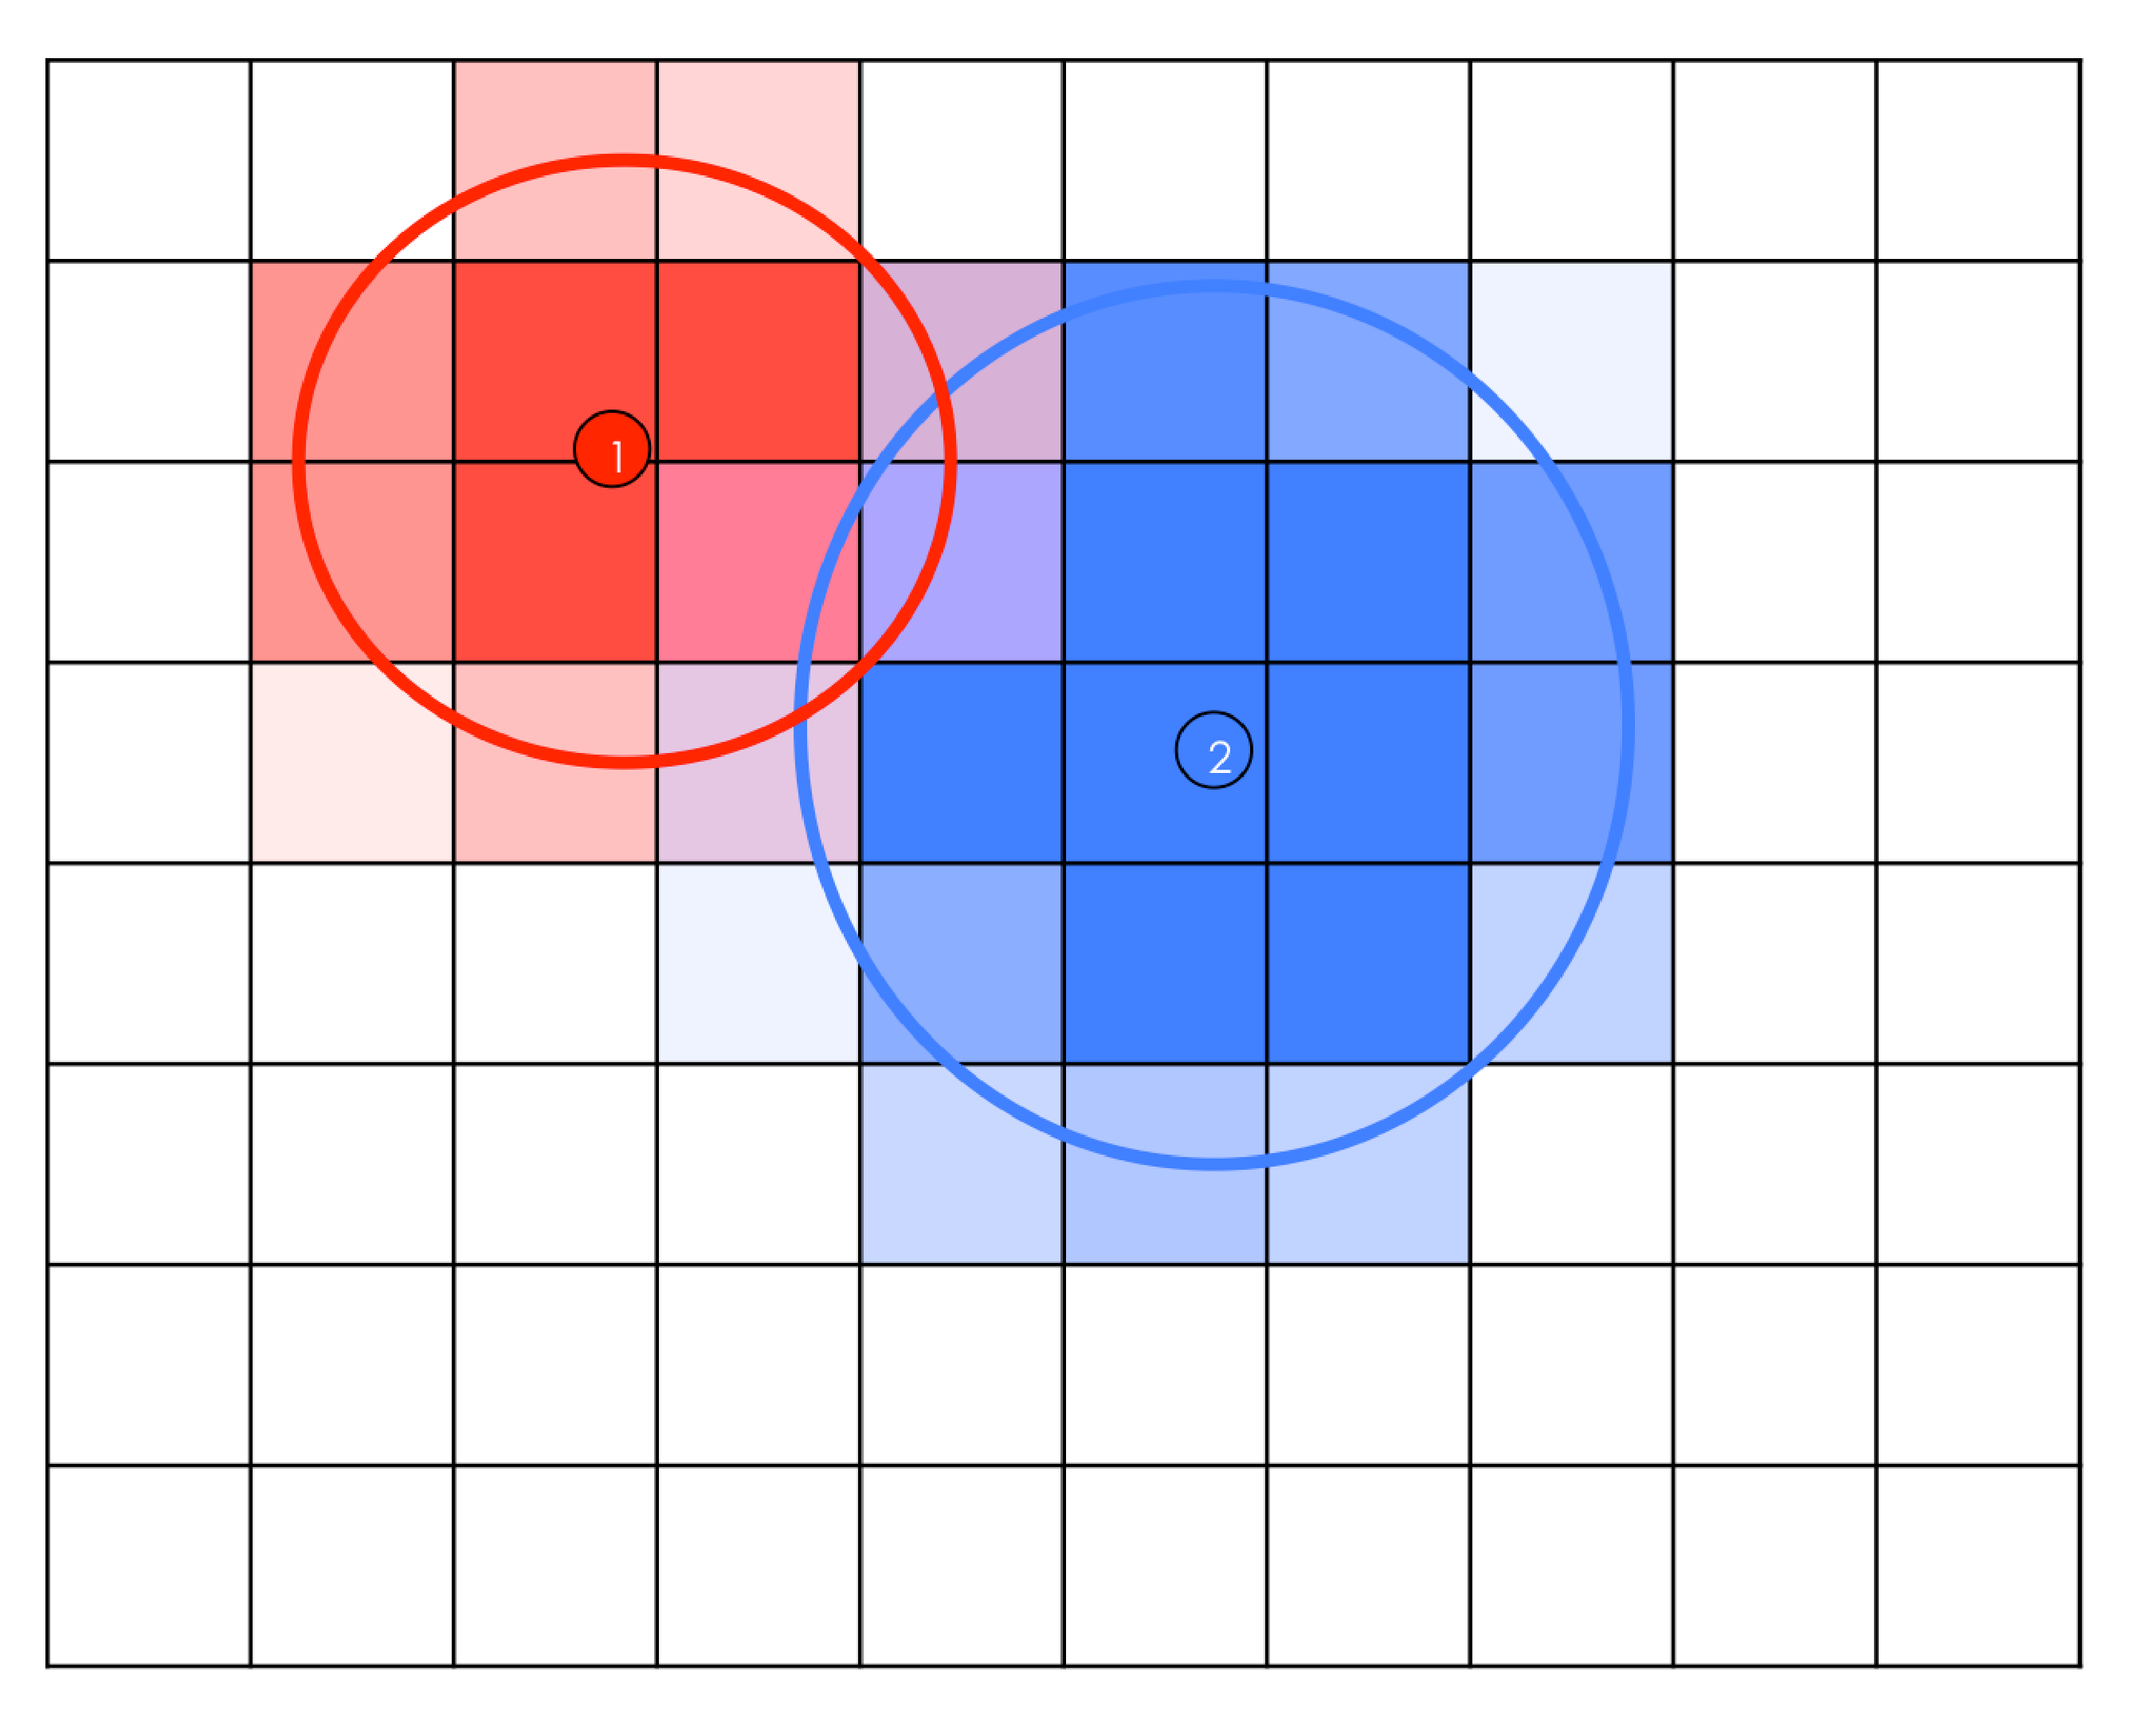
\includegraphics[scale=0.2]{images/particles.eps}
\caption{Two particles with different radii influencing the same pixels.}
\label{fig:particles}
\end{figure}


%\medskip
%\noindent
%{\bf Memory Access}
\subsubsection{Accessing Memory}
%\noindent
Data transfers between global and shared memory can be estimated 
as the sum of the number of loads 
GPU's global to shared memory plus number of stores from shared to global memory:
\begin{equation}
N_{Mgpu} = (N_{load,p} + N_{store,p}) N_{part} + N_{store,pix} N_{pix}^2,
\end{equation}
where $N_{load,p}$ and $N_{store,p}$ are the number of loads and stores of individual 
particles, and $N_{store,pix}$ is the number of stores of rendered images (no loads 
are expected since images are created on the GPU). 
Furthermore, memory access overheads can be estimated as $N_{Ngpu} \nu_{mem}$. $N_{Ngpu}$ is the overall number of memory accesses and $\nu_{mem}$ represents memory frequency. The overall times required for moving data among memories are thus calculated by:
\begin{equation}\label{tmgpu}
\begin{split}
T_{Mgpu} = {(N_{load,p} + N_{store,p}) N_{part} S_{part}
+ 12 N_{store,pix} N_{pix}^2\over \mu_{gpu}} + \\
+ N_{Ngpu} \nu_{mem} + g_{GPU},
\end{split}
\end{equation}
where $\mu_{gpu}$ is the global memory bandwidth
and $g_{GPU}$ the time 
spent on memory accesses by GPU specific functions. Equation \eqref{tmgpu} indicates that performances related to global-shared memory data transfers depend on $N_{load,p}$, $N_{store,p}$ - these quantify amounts of data transferred from global to shared memories and vice-versa. Achieved performances depend on memory bandwidth.

An optimal solution would be to realize a single data transfer only
(i.e. $N_{load,p} = 1$ and $N_{store,p} = 0$) with each thread processing a different particle fully. Such an approach ({\it one-thread-per-particle}) would guarantee optimal exploitation of GPU architectures. Nevertheless this is not practical, the main reason being that frequent race conditions may arise, 
as discussed above.
Only our {\it Rasterization} kernel is data parallel and can thus implement fully the {\it one-thread-per-particle} approach - in fact particles are processed independently. For this stage, $N_{load,p} = 1$ and since processed particles must be copied back to the global memory to be rendered $N_{store,p} = 1$. The {\it Rendering} kernel is envisaged to require an additional data load, but no more store 
stages are necessary (particles can be ``forgotten'' once their contribution is calculated).

For very large-scale datasets, the images size gives a meaningful contribution to $T_{Mgpu}$ only if the number of active particles (particles falling in the field of view, see Figure~\ref{fig:fov}) is of the same order of (or smaller than) the number of pixels. This can happen for specific camera settings.

A critical term in equation \eqref{tmgpu} is represented by the memory access
latency $N_{Ngpu} \nu_{mem}$. The access to memory is slow in comparison to
the available bandwidth, so a small number of accesses, $N_{Ngpu}$, is crucial
to performance. This can be achieved by standard caching strategies, that
however are effective only if data coalesced access (i.e. data are accessed by warps in one single memory transaction) can be guaranteed, in particular if consecutive particle data moved to the GPU L2 cache can be reused efficiently by consecutive threads. This is possible only through a global reorganization of the particle data, which has to be designed ensuring that no significant overheads are introduced and that overall linear scalability with the number of particles is preserved.

\section{CUDA Implementation}
\label{sec:implementation}

Once particles are loaded into the GPU's global memory, the {\it Rasterization} kernel starts processing them. We can follow an efficient {\it one-thread-per-particle} approach, so that the entire computation on individual particles (e.g. geometric transformation and coloring) is carried out by single threads - no interaction with any other processes is necessary. 
%This allows exploiting the underlying GPU architecture fully. (already stated before!) 
Subsequently the {\it Rendering} kernel takes over. As explained previously (see Section~\ref{sec:model}), for the rendering we cannot adopt a {\it one-thread-per-particle} approach. Moreover memory usage must be managed carefully.

To handle particles in an efficient way we observe that depending upon their radius ($r(p)$) as defined by equation \eqref{radius} rendering can be performed differently. As an example, since particles with a small radius typically influence single pixels on the rendered images, we can process these by deploying a {\it one-thread-per-particle} approach (see Section~\ref{sec:smallparticles}). On the other hand, particles with very large radius affect sizeable areas of the rendered images, so these are not suitable for efficient GPU processing (see Section~\ref{sec:largeparticles}). Finally, particles with radius within a suitably defined range influence only small fractions of the rendered images, so we process these by using a highly-efficient tiling strategy (see Section~\ref{sec:mediumparticles})

Therefore, we classify particles in three categories according to their radius as follows:

\begin{itemize}
\item
{\it Small (S)} : $r(p) \le r_{sml}$,
\item
{\it Medium (M)} : $r_{sml} < r(p) \le r_0$,
\item
{\it Large (L)} : $r(p) > r_0$.
\end{itemize}
where $r_{sml} = 0.5$ so that {\it Small} particles fall inside a single pixel, and 
$r_0$ is set according to the image tiling scheme which divides the rendered image
in a number of tiles:  
\begin{equation}
N_{tiles} = {N_{pix}^2\over t_x \times t_y},
\end{equation}
where $t_x$ and $t_y$ are parameters defining the sizes of tile sides in pixels.
%Details of the scheme are given in the next sections. 
An example of particle classification from different points of view is shown in Figure~\ref{fig:fov}.

Each particle is labeled (in the {\it Rasterization} kernel) with a {\it tile index} $i(p)$ as follows:
\begin{itemize}
\item
$i(p) = -2$, {\it non-active} particles (i.e. outside the field of view);
\item
$i(p) = N_{tiles}$, {\it small} particles;
\item
$0 \le i(p) < N_{tiles}$, {\it medium} particles, whose center falls in the $i(p)$-th tile;  
\item
$i(p) = -1$, {\it large} particles.
\end{itemize}

Subsequent to classification we transfer asynchronously all large particles back to the host and remove them together with all inactive ones from the device memory. At this point, the remaining particles have to be sorted by the $i(p)$ key and the number of particles with the same index has to be calculated.
%At the end of this operation, all particles with the same tile index are contiguous in memory,
%providing an optimal memory access pattern and can be easily isolated for tiles assignment and processing.
%A specific kernel has been developed to implement these operations.
This sorting operation is important as it allows to manage particles array on the device and it is  
necessary for the efficient execution of subsequent operations, e.g. reduction by key and prefix sums.
%, because memory accesses to the array elements involved in a CUDA operation are efficient when consecutive threads access consecutive elements.

As sorting is intrinsically an expensive operation, we use an efficient implementation provided by the Thrust library \cite{thrusturl}. Thrust is a C++ template library for CUDA which mimics the Standard Template Library and provides optimized functions for managing very large data arrays. For our purposes, Thrust implements a highly optimized Radix Sort algorithm for primitive types (e.g., chars, ints, floats, and doubles). Also, functions are provided for reduction by key and prefix sums, their performance increasing the larger the input data arrays. As these functions scale linearly with data sizes (sorting scales by $kN_{part}$, where $k$ is the number of significant key bits \cite{RadixSort}), our GPU implementation preserves Splotch's overall linear dependency on the number of input particles. The sections below describe the rendering details for individual classes ({\it small}, {\it medium}, {\it large}) of particles.

\begin{figure}
\centering
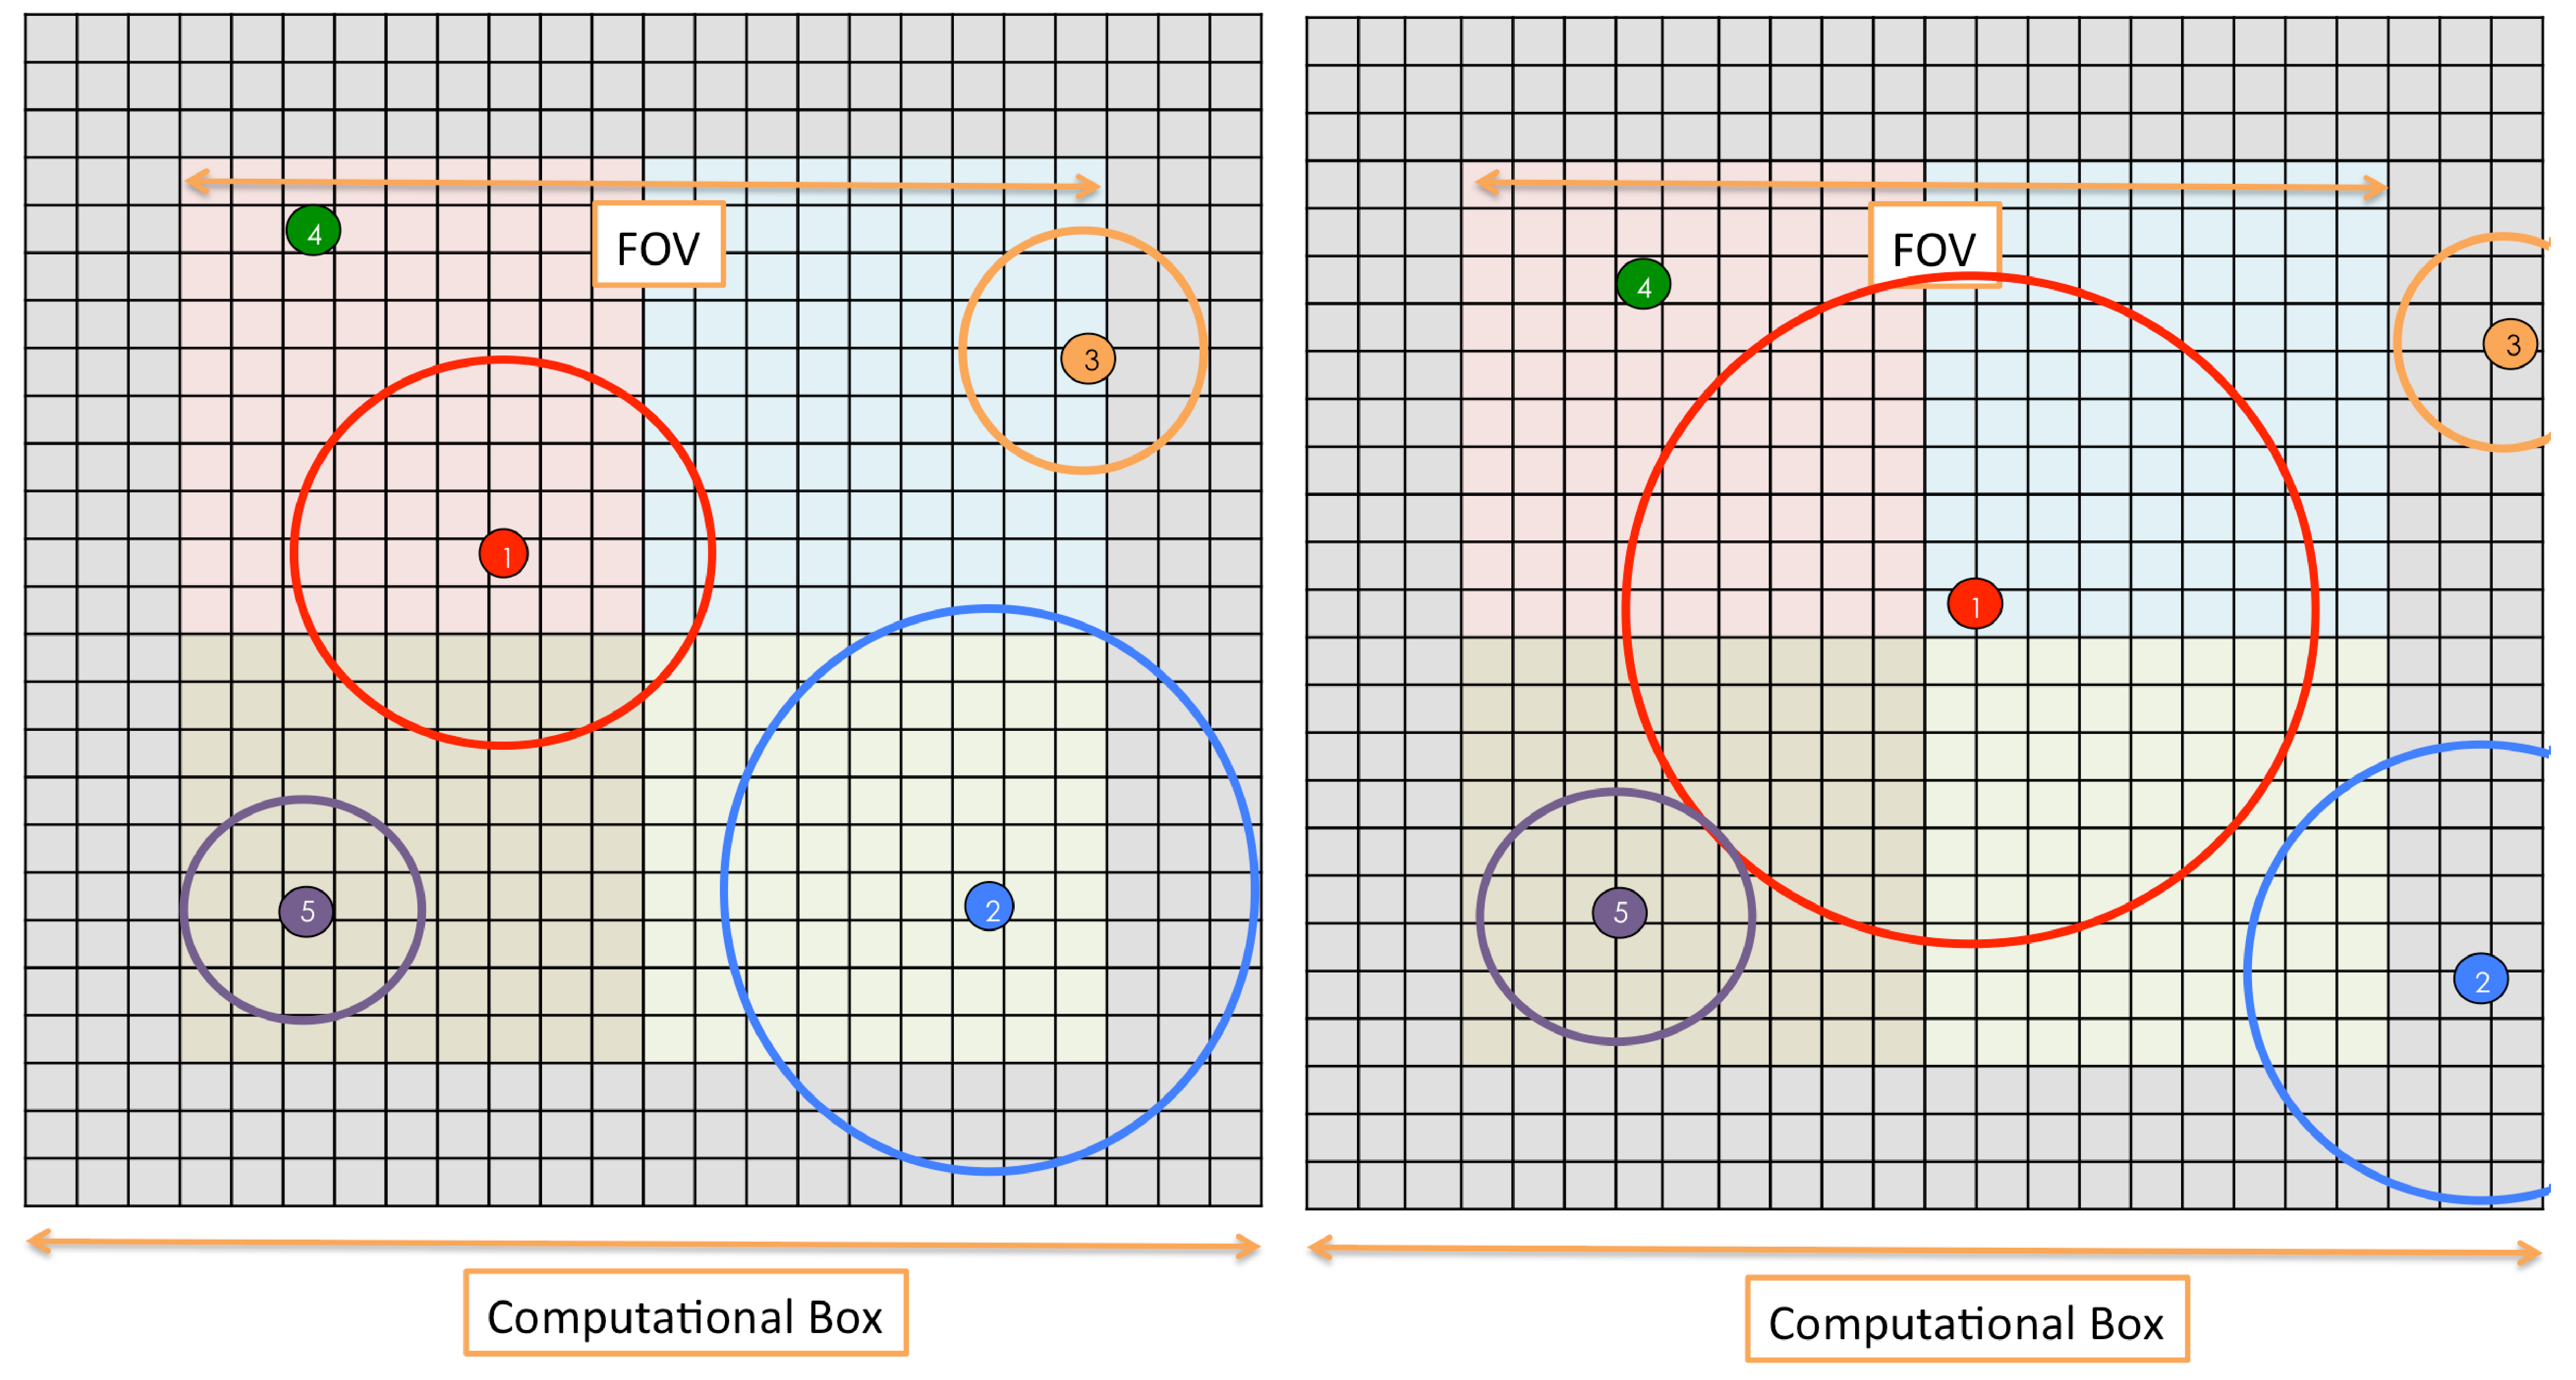
\includegraphics[scale=0.15]{images/fov.eps}
\caption{The scene with five particles from two different points of view. Different square tiles are
represented with different colors and boundary width is $r_0=3$ pixels. {\em Left}: All particles contributes to the image (lie in the FOV), particles 1, 3 and 5
are medium, particle 4 is small. Particle~2, is classified as large since its radius exceeds the boundary width. {\em Right}: The camera moved toward particle~1. All the radii change due to the new point
of view. Classification of particles 4 and 5 does not change, while particle~3
becomes inactive (completely falling outside the FOV). Particle~2, though
having coordinates outside the FOV, affects some pixels, hence it is still active.
Particle~1 becomes large.
}
\label{fig:fov}
\end{figure}

\subsection{Small Particles}
\label{sec:smallparticles}
Only the position of individual particles within rendered images has to be calculated. This can be efficiently carried out by assigning CUDA threads to particles. However, since different threads can affect the same pixel in the rendered images, their contribution (fragments) cannot be directly accumulated. Thus firstly we allocate a buffer (index buffer) in the device memory to store particle positions. Secondly, the image is updated by reducing by key (pixel position) all fragments - these are equal to the color associated to particles from rasterization - and adding each pixel contribution to the image.
%Particles are sorted by pixel id followed by reducing contiguous elements falling on the identical pixels using functions from the Thrust library.

\subsection{Medium Particles}
\label{sec:mediumparticles}
Our \textit{tiling scheme} for rendering medium particles on the device consists of assigning particles related to the same image tile to a block of CUDA threads and exploiting the shared memory and thread synchronization within the block to store and compose image tiles. The local size of the tile is defined so that each particle belonging to it, is entirely contained within the tile. This is achieved by adding to the $body$ of the tile of $t_x \times t_y$ pixels a $boundary$ of $r_0$ pixels around it (see Figure~\ref{fig:fov}). We will refer to this extended tile as a \textit{Btile}.

Particles are accessed in chunks of $n_p$ elements. Each chunk is accessed and stored in the shared memory by a single read operation, performed simultaneously by the threads of the block. Then, the particles of the chunk are rendered sequentially, each with a single parallel operation so that each pixel of the particle is processed by a different thread of the block (the pixel number processed by each thread may change as the particle varies, but it remains in the Btile). The block dimension is equal to the size of the biggest medium particle (i.e.~$4r_0^2$), in order to have enough threads of the block for rendering each pixel of the current particle. 
This solution avoids race conditions when composing the image tile, since each
thread of the same block accesses different pixels. Moreover the workload of each
thread is well balanced because each thread processes either one o no pixels for each particle, independently of the particle size. 

When all particles of the block are rendered, the contribution of the Btile is added to the image stored in the global memory. Specific care has been taken to avoid race conditions due to contributions coming
from overlapping regions (boundaries). Since CUDA blocks are order independent, three more copies of the image in the global memory are necessary to store corners, rows and columns of the boundary respectively. The final rendered image is then obtained by executing a follow up kernel compositing these copies.

Note that, even if the OpenMP implementation use a tiling scheme these two approaches are quite different. While large particles can be split among different tiles in the OpenMP version, this solution is much more complicated for CUDA because particles falling in several tiles must be replicated for each tile affected by them and added to particles array. For this reason we have been able to render on the device only particles completely contained in one single tile extended with a suitable boundary. 

\subsection{Large Particles}
\label{sec:largeparticles}
Large particles are the most challenging to process as their large
radius prevents the usage both of a tiles based solution and of a fragment buffer.
In the first case, tiles would be too large to be stored in the shared memory
and, in any case, their large overlap could lead to strong overheads in the composition of the
final image. Using a fragment buffer instead would require too much memory, since
for each particle a large number of fragments would be generated, possibly
larger than the available memory. Our solution to these problems is to copy these particles back to the CPU and performing their rendering
using the serial version of Splotch. This is possible thanks to CUDA asynchronous
operations, which allow to copy data from the device to the host (and vice-versa)
whilst the calculation on the GPU is on-going. Once the particles are back to the CPU,
their processing can be performed concurrently to that of the GPU.  
This way, we manage to exploit both the host and the device simultaneously.
This solution is effective as long as the number of large particles
is much smaller than the sum of small and medium particles. As a worst case scenario (although highly unlikely in practise), if all particles are classified as large, the rendering performance would degenerate to that of the serial implementation of Splotch.

Once all calculations are completed, the two partial images (one processed by the GPU the other by the CPU) are composed to generate the final rendered image. Such operation is performed by the CPU, once the GPU partial image has been transferred, with a single copy operation, to its memory. 

\subsection{Discussion}
For both small and medium particles the main drawback of the proposed solutions
is represented by the overhead associated with the sorting and reduction operations. In particular the sorting is intrinsically time-consuming, requiring intensive memory usage.
The performance of the approach for rendering medium particles is mainly influenced
by the size of the shared memory, which limits the number of resident blocks
per multiprocessor during the execution of the kernel, thus reducing the device occupancy. 
%(see Section~\ref{sec:gpuperf}).
A further issue is related to the unbalanced work load among blocks. In fact the number of particles falling in each tile can vary in a significant way from one tile to another. All these aspects will be quantitatively analyzed in the next section.

\section{Results}
\label{sec:results}

%\begin{figure}
%\centering
%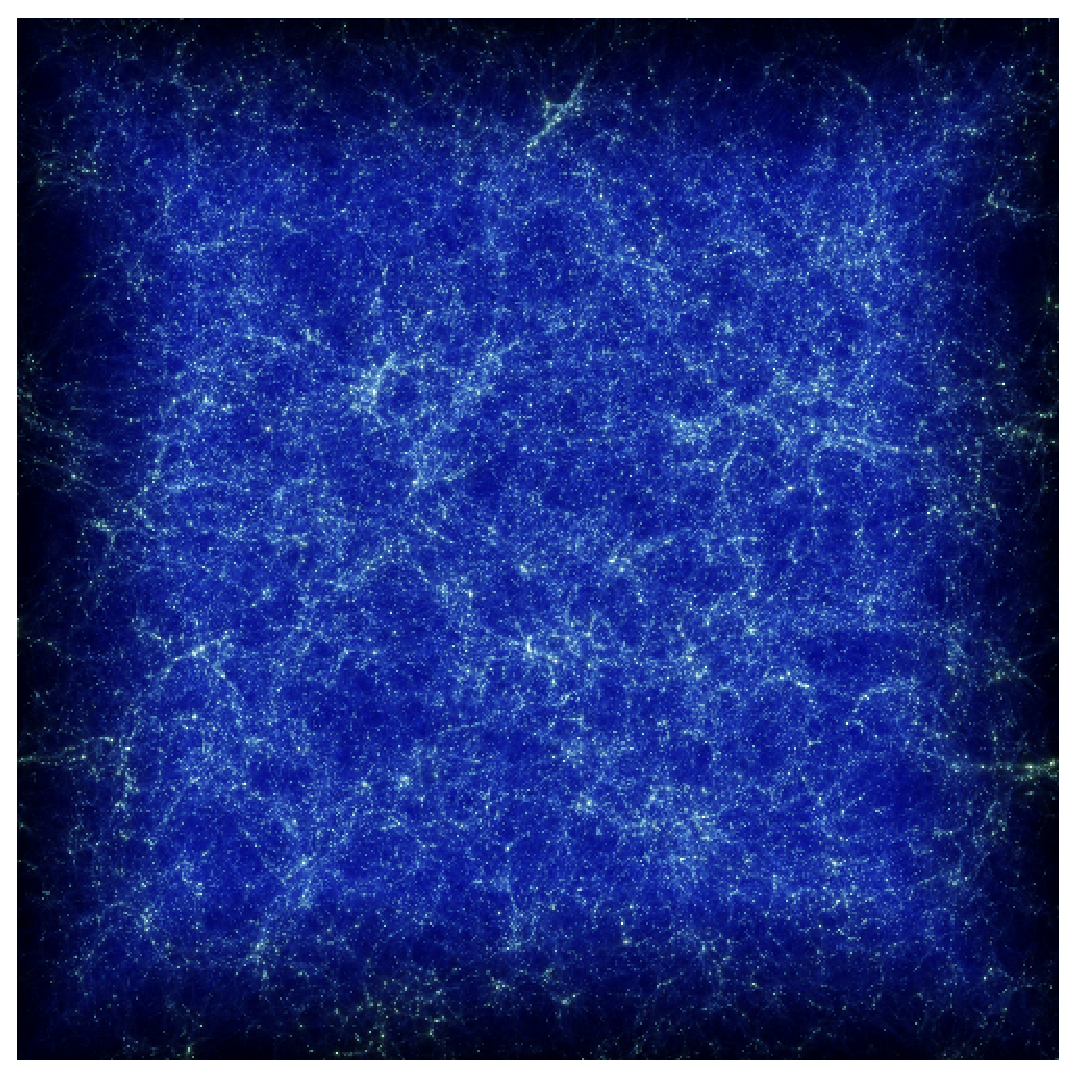
\includegraphics[scale=0.6]{images/box.eps}
%\caption{Mass distriN-body cosmological simulation }
%\label{fig:box}
%\end{figure}

An N-body simulation performed using Gadget \cite{gadgeturl} was used for the tests we discuss in this section. The simulation is based on about 400 million particles consisting of 200 million {\it dark matter} particles, 200 million baryonic matter particles (hereafter referred to as {\it gas}) and around 10 million {\it star} particles. Particles possess a number of physical quantities, e.g. vectors capturing spatial coordinates and velocities, or scalars representing smoothing length. Additionally gas particles are associated with {\it temperature} and {\it mass density}. Also, {\it spectral type} and {\it age} are properties of star particles. Such quantities can be exploited in highly-detailed renderings, e.g. for modulating colors and intensities appropriately. 

We used GCC 4.4.6 and CUDA 5.0 for compilation. Execution was performed on a computing node containing a dual-socket six-core Intel Xeon 5650 2.6 GHz processor with 24 GB shared memory and a pair of NVIDIA Tesla M2090 GPUs with 6 GB of GDDR5 memory, 177 GB/sec main memory bandwidth and peak performance of 665 GFlops/sec. Although such a large memory computing node is necessary for handling our test simulation ($\approx 7.5$ GB) no GPU issues arise as data is loaded in small chunks iteratively. This section presents a performance analysis of our GPU implementation and compares to the parallelized CPU version of Splotch. 

\subsection{Tuning}
\label{sec:gpuperf}
To perform the tests presented in this section an important aspect is ensuring high {\it occupancy} by exploiting underlying GPUs appropriately so as to avoid the situation in which cores remain idle during kernel execution. Occupancy depends upon the number of threads per block, the number of registers and the size of shared memory used in a kernel - as these define the number of resident CUDA blocks (blocks/SM) during execution. We have empirically estimated a good trade-off among these parameters for the rendering kernel of our implementation. This kernel may potentially use significant shared memory due to the fact that Btiles together with a number of particles need to be stored. As the boundary width of Btiles is critical for realizing particle classification and for determining sizes of CUDA blocks, we suggest to fix this no larger than 8, because of the small shared memory size, and focus instead on optimizing the relevant number of particles ($n_p$) and the size of tiles (for simplicity we consider square tiles of size $t_x^2$) respectively.
 
Notice that the tile size is also relevant to the load balancing among different blocks: as the tile size decreases the work load is less unbalanced. 
%However this problem cannot completely overcome when the dataset distribution is heterogenous at all scales. Therefore a further investigation must be done for this issue.

A number of possible $n_p$ and $t_x$ values are illustrated in Table~\ref{tab:tuning}. We considered the situation in which the majority of particles is non-large so that they are processed by the GPU. This way we obtain meaningful rendering times for our optimization as the host computation is overlapped by the device computation completely. We observe that storing Btiles together with a fixed number of particles in shared memory (for optimizing memory access) restricts full GPU occupancy. The maximum occupancy obtained is $66.7\%$ for small tiles ($t_x = 10$ or $t_x = 12$) and small chunks of particles ($n_p = 32$ or $n_p=64$). Taking into account total CUDA times, optimal performance is achieved for $n_p=64$ and $t_x = 12$, so we employ these values for testing in the next sections.

\begin{table}
\label{tab:tuning}
\begin{center}
\begin{tabular}{|l|l|l|l|l|}
\hline
$n_p$ & $t_x$ & Kernel & Rendering & Total CUDA \\
& & Occupancy & Times (sec.) & Times (sec.) \\
\hline
256   & 16 & 0.333 & 9.186 & 16.38 \\
\hline
      & 14 & 0.333 & 7.345  & 15.30 \\
\hline
      & 12 & 0.333 & 6.881  & 14.01 \\
\hline
      & 10 & 0.333 & 6.768 & 14.06 \\
\hline
128   & 16 & 0.333 & 9.159 & 17.00 \\
\hline
      & 14 & 0.333 & 7.302  & 15.30 \\
\hline
      & 12 & 0.5 & 5.074  & 12.08 \\
\hline
      & 10 & 0.5 & 5.016 & 12.30 \\ 
\hline
64    & 16 & 0.5 & 6.516 & 14.23 \\
\hline
      & 14 & 0.5 & 5.387 & 12.55 \\
\hline
      & 12 & 0.667 & 4.423 & 11.34 \\
\hline
      & 10 & 0.667 & 4.393 & 11.45 \\ 
\hline
32    & 12 & 0.667 & 4.515 & 12.41 \\
\hline
      & 10 & 0.667 & 4.483 & 12.43 \\ 
\hline
\end{tabular}
\caption{The rendering times obtained for different values of $n_p$ (number of particles) and $t_x$ (tile side). Square tiles with boundary 8 are considered while the resolution of rendered images is $1024^{2}.$}
\end{center}
\end{table}

\subsection{Performance Analysis}
\label{sec:performance}
This section discusses performances of our implementation in terms of scalability with the sizes of datasets and rendered images (Section~\ref{sec:scalability}), comparison with the CPU version (Section~\ref{sec:speed-up}) and the GPU overhead (Section~\ref{sec:overhead}).

\subsubsection{Scalability}
\label{sec:scalability}
To analyze scalability in terms of sizes of datasets objectively we fixed the size of rendered images and camera settings so that all particles are classified as non-large and are thus processed by the GPU entirely. 
Figure~\ref{fig:scalability} illustrates the obtained timings when progressively increasing the overall number of particles
from about $10^7$ to roughly $2.2\times 10^8$. Computing times scale linearly confirming that our implementation preserves this essential feature of the original CPU Splotch. 
\begin{figure}
\centering
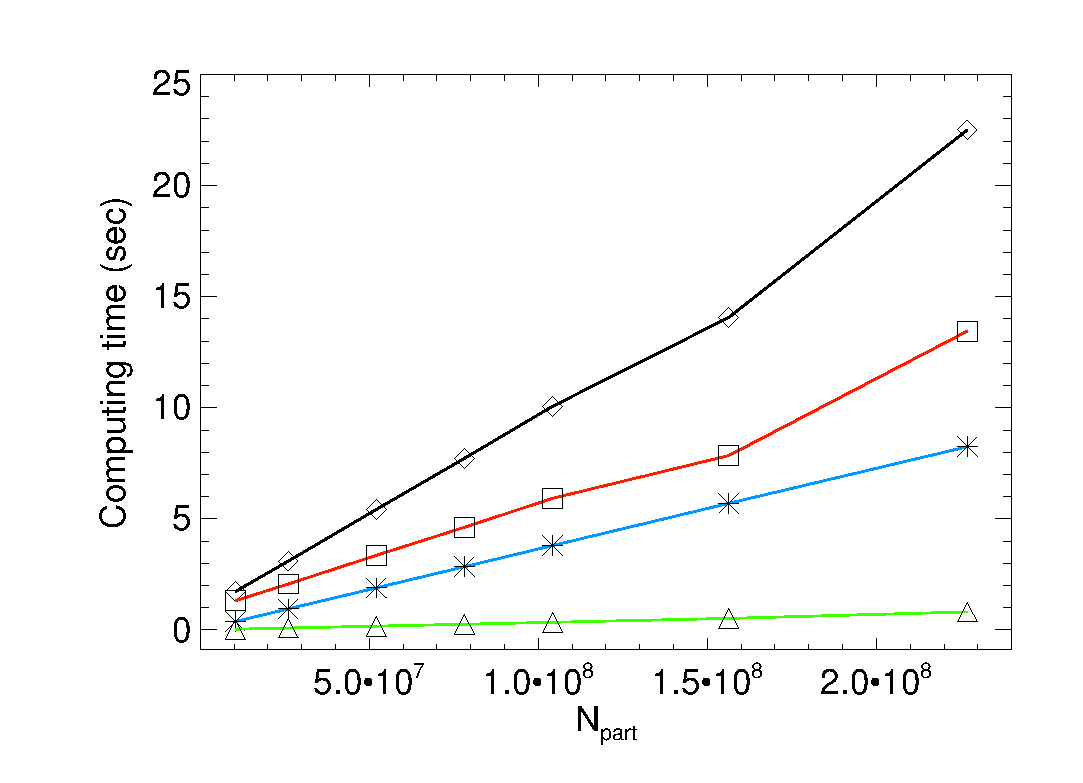
\includegraphics[scale=0.5]{images/scalan.eps}
\caption{Scalability of Splotch kernels on the GPU in relation to dataset sizes. 
The black line (diamonds) shows total computing times, the red line (squares) shows rendering times, the blue line (crosses) represents the Overhead times and the green line (triangles) shows the Rasterization times.}
\label{fig:scalability}
\end{figure}

%OPEN
%CLAUDIO: I suggest to add the meaning of the y-axis in the plot, i.e. computing time 

We observe a perfect linear scalability of the rendering times with $N_{part}$, 
these representing one of the two main contributions to overall computing times, 
the other being the sum of the overheads related to all those parts specific to the GPU code 
refactoring (e.g. times for host-device copy or distribution of particles - see Section~\ref{sec:overhead}). 
Rasterization requires instead a negligible fraction of the overall time (5\% to 10\%). 

%\subsubsection{Image Sizes}
%\label{sec:imagesizes}
Overall performance in relation to image sizes $N_{pix}^2$ is illustrated in Figure~\ref{fig:pixels}. Keeping the underlying dataset size and camera settings fixed, we obtained computing times by progressively increasing
$N_{pix}$ from 128 to 4096. According to \eqref{ops} and \eqref{radius} each particle contributes to a number of pixels that is proportional to $N_{pix}^{2}$. As long as image sizes are small relative to dataset sizes (for our particular configuration this translates to $N_{pix} \le 1024$), overall computing times are constant. For large image sizes their resolution may affect significantly the classification of particles potentially increasing overall computing times dramatically.

\begin{figure}
\centering
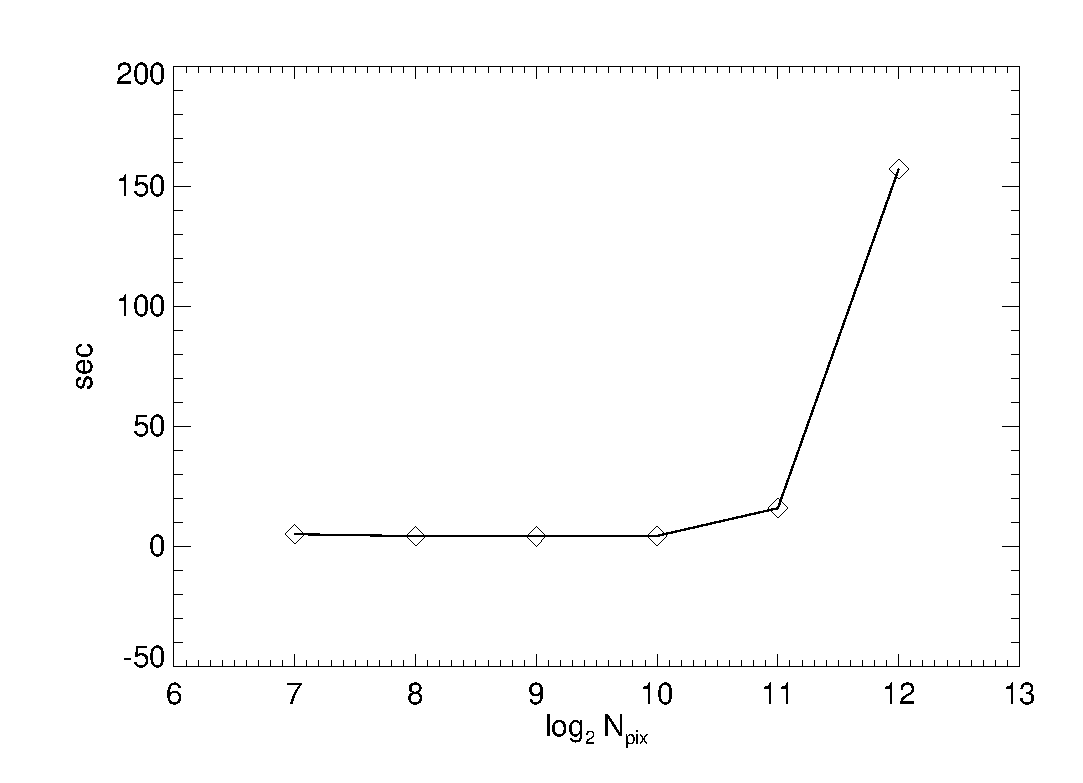
\includegraphics[scale=0.5]{images/pixels.eps}
\caption{Splotch's scalability on the GPU in relation to image side $N_{pix}$ (camera settings are fixed).}
\label{fig:pixels}
\end{figure}

%OPEN
%CLAUDIO: I suggest to add the meaning of the y-axis in the plot, i.e. total computing time

\subsubsection{Speed-up}
\label{sec:speed-up}
In the next series of tests, we discuss the speed-up achieved with respect to the CPU performance. 
The dependency of the computing time from the radius, defined by equation \eqref{radius}, has been analysed keeping 
the image resolution fixed ($N_{pix} = 1024$) and progressively changing the camera position 
so as to resemble a typical user interaction scenario, namely a zoom in operation. 
The starting camera position ensures that the entire box of the simulation is rendered (Test 1). 
Next we ensure that the simulation box just about fits into the rendered images (Test 2). 
A few other camera positions have also been set so as to reach closer and closer towards the 
centre of the simulation (Tests 3 to 7). Figure~\ref{fig:panorama} illustrates rendered images 
generated for the different camera positions.
We observe that approaching the center of the simulation results in larger radii 
as expressed by the average $R_0=<r(p)>$ radius and illustrated by Figure~\ref{fig:radii}. 
Table~\ref{tab:radius} shows these values together with the number of active particles and computing times. 

As we approach the centre of the simulation fewer particles are active, an increasingly larger 
fraction falling outside the scene. This leads to a reduction in the computing time. At the same
time, however, particles are closer to the camera and their radius increases contributing to 
a progressively larger number of pixels,
thus increasing computing times with the square of their radius. 
These two opposte trends tend to compensate keeping overall times from 10 to 16 seconds.

\begin{figure}
\centering
\includegraphics[scale=0.2]{images/panorama.eps}
\caption{The adopted test particle simulation as rendered by Splotch at a number of different camera positions mimicing a zoom-in operation: starting from very far (top-left image) and reaching very close to the center of the simulation. Particles' mass distribution is shown.}
%OPEN
%CLAUDIO - HERE AS DISCUSSED IT WOULD BE GOOD TO SHOW THE ZOOM IN, PERHAPS A SMALL RECTANGLE THAT BECOMES LARGER TO SHOW THE AREA WITHIN WHICH WE ZOOM IN
%ANSWER: I'LL DO THAT IN THE NEXT DAYS
\label{fig:panorama}
\end{figure}

\begin{figure}
\centering
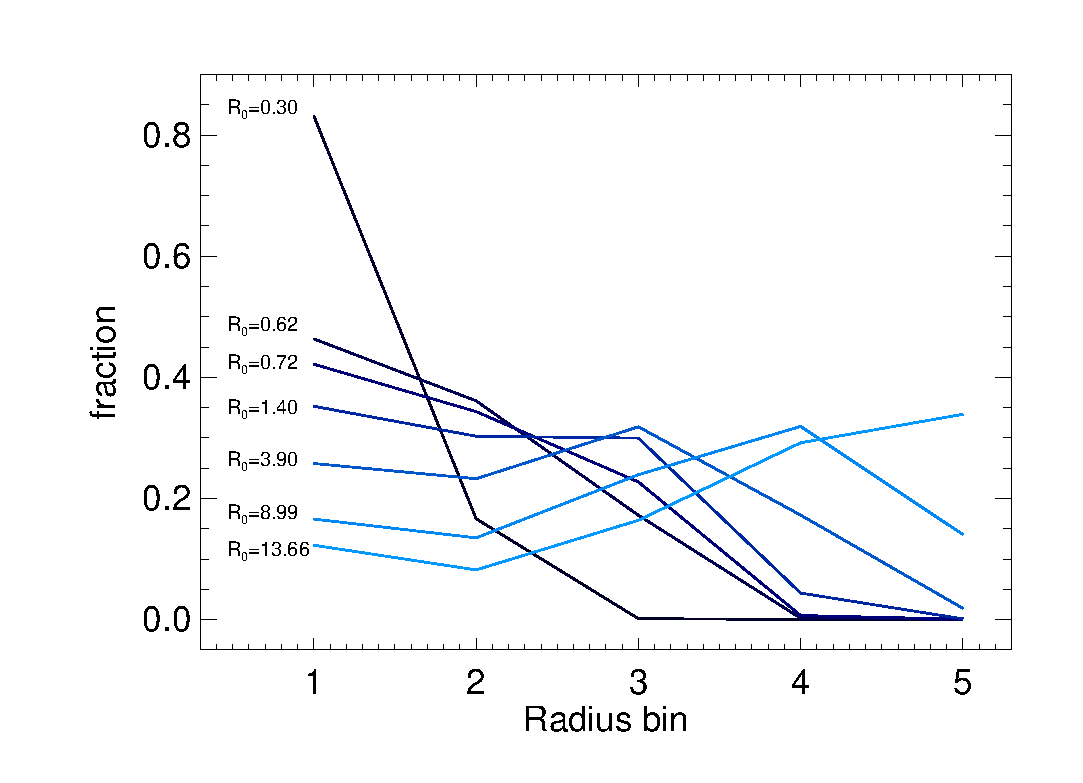
\includegraphics[scale=0.5]{images/radii.eps}
\caption{Fractional distribution of the particles radii in the seven tests (dark blue line refers to Test 1, light blu to Test 7). Radius bins in the x-axis corresponds to: $r\le 2$ (bin~1), $2<r\le 4$ (bin~2), $4<r\le 8$ (bin~3), $8<r\le 16$ (bin~4), $r>16$ (bin~5). 
}
\label{fig:radii}
\end{figure}

\begin{table}
\begin{center}
\begin{tabular}{|l|l|l|l|}
\hline
Test ID & $R_0$ (pixels) & Active Particles & Time (sec.) \\
\hline
Test 1  & 0.30   & 226894837  & 12.89 \\
\hline
Test 2  & 0.62   & 225972201  & 12.52 \\
\hline
Test 3  & 0.72   & 212746328  & 12.20 \\
\hline
Test 4  & 1.40   & 153647633  & 10.05 \\
\hline
Test 5  & 3.90   & 64756141   & 14.85 \\
\hline
Test 6  & 8.99   & 13686588   & 16.11 \\
\hline
Test 7  & 13.66  & 4222214    & 12.75 \\
\hline
\end{tabular}
\end{center}
\caption{Illustration of average particle radius (column 2) together with number of active particles (column 3)
and computing times (column 4) for each performed test (test ID is presented in column 1).}
\label{tab:radius}
\end{table}

%\subsection{Discussion}
%\label{sec:discussion}
CPU Splotch timings were obtained exploiting the OpenMP paradigm on 1, 2, 4, 8 and 12 processors respectively. OpenMP was selected (instead of MPI) as the design of this parallelized CPU Splotch is conceptually closer to our CUDA implementation (see Section~\ref{sec:overview}). The results are illustrated in Figure~\ref{fig:gpucpu} as a function of computing times per particle, since the number of processed particles depends on camera settings.

\begin{figure}
\centering
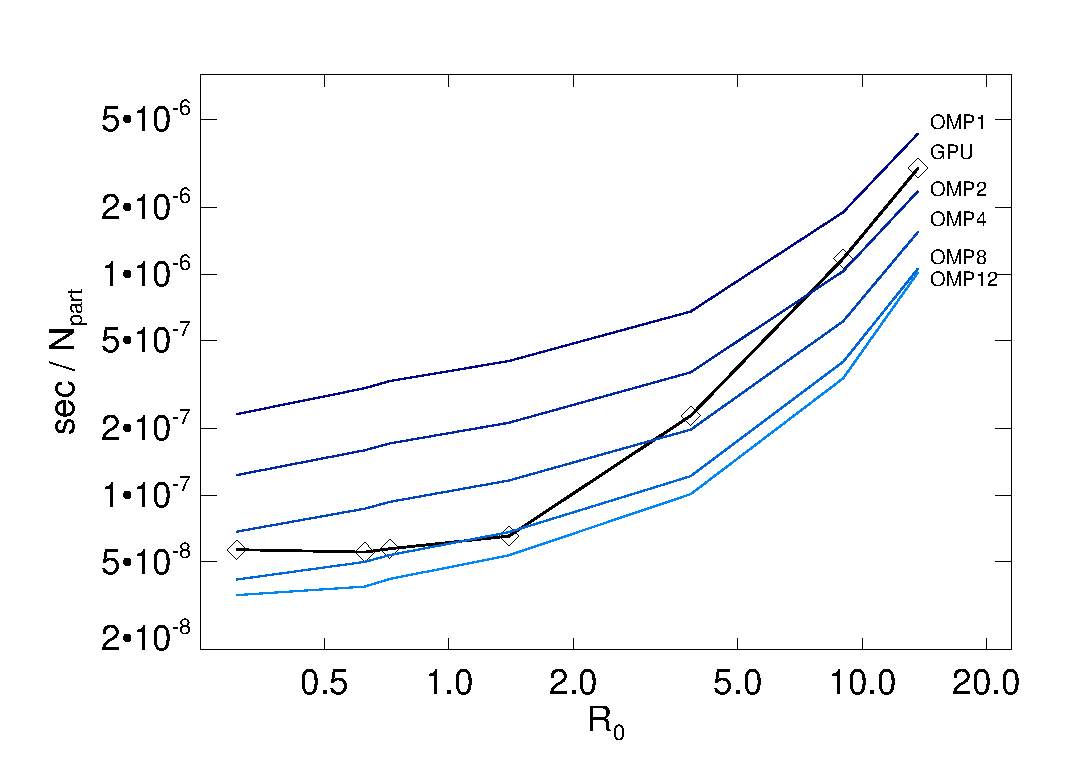
\includegraphics[scale=0.5]{images/scalaomp.eps}
\caption{GPU and CPU comparison in relation to the particles' radius. The black curve represents GPU computing times. Blue curves are CPU times ranging from 12 cores (light blue, OMP12) to 1 core (dark blue, OMP1).}
\label{fig:gpucpu}
\end{figure}

\begin{figure}
\centering
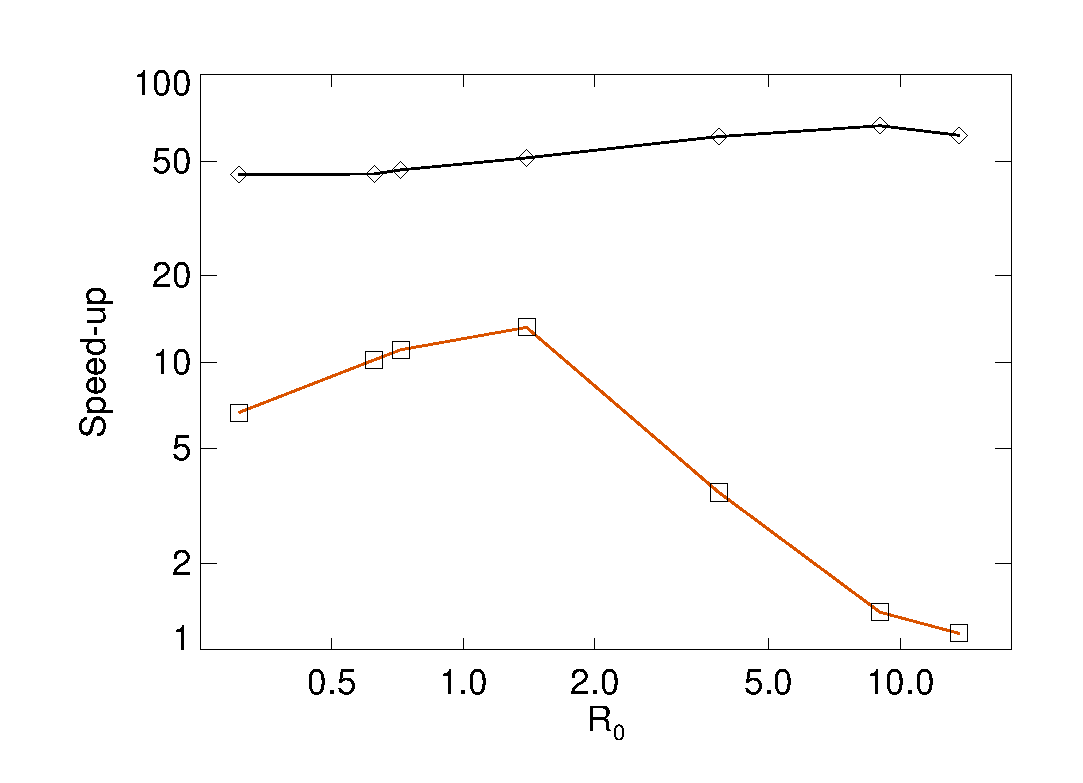
\includegraphics[scale=0.5]{images/speedup.eps}
\caption{
Observed speed-ups for rendering (red curve, squares) and rasterization (black curve, diamonds) kernels defined as ratios among computing times required for execution by the GPU and CPU respectively.
}
\label{fig:speedup}
\end{figure}

The GPU curve exhibits a bi-modal behaviour depending upon the radius. For small values, computing times are almost constant since the overall calculation is dominated by $N_{part}$. For values larger than unity the dependency from the square of the radius dominates and computing times rise rapidly. The comparison between the GPU and the multicore performance show that at small radii ($R_0 < 2$) the speed-up gained by the GPU implementation can be larger than a factor of 6 compared to a single CPU. Considering the OpenMP implementation of Splotch we observe that within this range of radii, GPU performance is comparable to that obtained from 8 cores. This is because parallel codes do not scale linearly with the number of processors. At large radii ($R_0 > 2$) the performance of CUDA deteriorates naturally as the majority of particles is CPU processed. Nevertheless assuming a worst case scenario GPU Splotch is always faster than single core execution. 

We conclude this section with a discussion on the performance achieved by all GPU kernels implemented. 
We compare computing times required for rasterization and rendering on the 
GPU and CPU respectively (See Figure~\ref{fig:speedup}). 
As regards the rendering kernel, a speed-up of around 13 is obtained for average radii around unity. For smaller radii the speed-up
tends to decrease due to the lower occupancy of the rendering kernel processing medium particles.
In fact, from Figure~\ref{fig:radii}, one can see that for $R_0<1.4$ most of the medium particles have a radius lower than the threshold~$r_0=8$ defining the size of CUDA blocks, therefore several threads in each block do not process any pixel.
As the radius grows, performance decreases due to the increasing number of large particles.
Regarding the rasterization kernel due to the {\it one-thread-per-particle} approach it is strongly accelerated with observed speed-ups ranging from 45 to 65.  

\subsubsection{Overheads}
\label{sec:overhead}
Finally, we discuss the GPU overheads, i.e. times required by functions specific to our GPU implementation. To this extend a number of operations are necessary, e.g. for offloading particles to GPU (OffLoad), sorting and reducing for preparing Btiles and optimizing memory displacement (Sort), removing non active particles, packing and copying back particles that have to be rendered by the CPU (Select) and finally, performing partial images composition. Figure~\ref{fig:over} presents the overhead of different GPU specific functions as times spent by the function divided by overall computing times. The black curve shows total overheads which can be up to 60\% and particularly significant for small radii. As most of the particles are active the sort and reduce 
functions (blue line with crosses) are heavy. For large radii this overhead is negligible as most of the particles are inactive. 

\begin{figure}
\centering
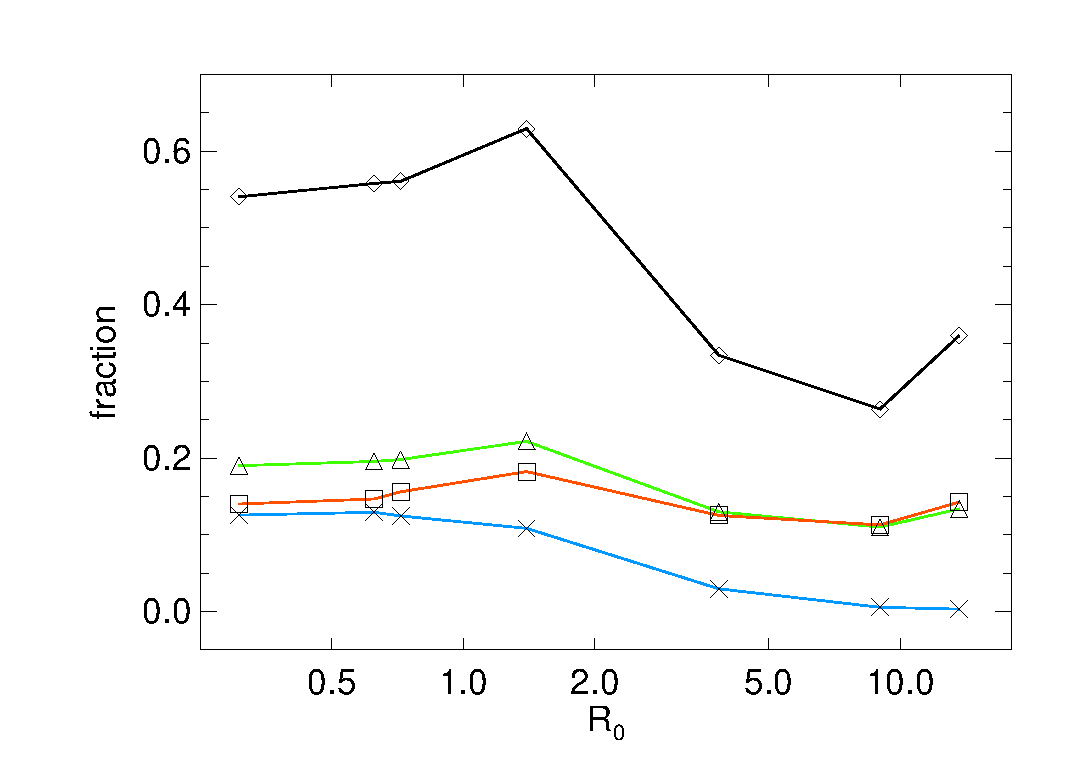
\includegraphics[scale=0.5]{images/over1.eps}
\caption{Overhead of the various components implemented for the Splotch's
GPU refactoring. The ratio between the time spent in each component and the total processing 
time is shown. The black line (diamonds) shows total overhead, the green line (triangles) shows the Select time overhead, the red line (squares) represents the OffLoad time, the blue line (crosses) shows the Sort time.}
\label{fig:over}
\end{figure}
%OPEN
%CLAUDIO - Are you sure of the last point of the black line in the picture above? I think it is wrong....

The red curve represents offload times which are constant in our tests (as all particles are moved to the GPU irrespectively of camera position), about 15\% of overall overheads. This contribution tends to decrease at larger radii due to the increased overall processing times. The Select times are slighlty higher than that of OffLoad and this tends to decrease at larger radii, when more particles are moved back to the CPU, hence coalesced memory access can be effectively exploited. Finally, image composition (and any other CUDA set up times) can always be considered negligible contribution, e.g. creating rendered images accounts for approximately 0.1\% of GPU overheads. This is due to the efficient design of our implementation which takes full advantage of the multi-thread architecture 
of the GPU.
%OPEN
% MARZIA - NEED TO EXPLAIN A LITTLE MORE HERE, about the 0.1% TO JUSTIFY. ALSO WHAT WOULD THE PERCENTAGE BE FOR THE SETTING UP CUDA OVERHEAD?
% ANSWER: I WOULD REMOVE THIS PART, IT IS NOT RELEVANT AND IT IS NOT REPORTED IN THE PLOT


\section{Conclusions and Future Developments}
\label{sec:conclusions}
The CUDA implementation of Splotch allows to exploit GPUs 
for the visualization of huge data volumes, such those produced both 
by experiments/observations and by computer simulations. Current trends
in HPC envisage the adoption of accelerators to substantially 
increase the performance of the computing systems, maintaining the power
consumption reasonably low. However, accelerators, and in particular 
GPUs, requires a certain effort to be efficiently exploited, 
supporting only peculiar programming models, that requires codes, or part
of them, to be redesigned and reimplemented before being suitable to such devices. 

Splotch proved to be a challenging application to enable to GPUs. 
In fact, the main computational kernel, the Rendering kernel, poses serious difficulties
to the GPU's programming model, that privileges highly data parallel algorithms.
In order to overcome such difficulties, Splotch's rendering algorithm has been
redesigned with the introduction of specific kernels. These kernels 
introduce an overhead that can be up to the 60\% the overall computing
time. Nevertheless, the final code overperforms the original CPU
version of up to a factor of 6, which rises to a factor of 8 when the OpenMP,
multithread parallel version is considered for comparison. Further optimization can
be obtained by the adoption of CUDA streams, overlapping computation 
and data movements. However this is currently prevented by the rendering of large particles on the CPU and the usage of the Thrust library that do not support such kind of operational mode. 
The Splotch GPU code retains also an important feature of the original
code: the linear scalability with the number of particles.
% THIS IS WRONG: and with the image size. 

Although not extraordinary, the attained GPU performance is sufficient 
to run efficiently on the hybrid computing nodes that are more and 
more common in the HPC framework. In order to fully exploit such architectures, 
a further step is necessary, supporting the concurrent usage of 
multiple GPUs, multiple cores and multiple nodes, exploiting respectively the OpenMP and
MPI capabilities of Splotch. This step is expected to pose important 
challenges especially to find the optimal balance in the workload of each of the different 
system components.

Although GPUs offer an excellent platform for improving performances of numerical codes, a complete redesign of algorithms is often necessary and dramatic improvements cannot be guaranteed. Nevertheless, even when moderate performance gains are achieved, GPU enabled codes allow full exploitation of modern HPC systems combining multicore processors with multiple GPUs. 

%In principle, this overhead could
%be strongly reduced adopting CUDA streams and overlapping data copy to
%computation. However, this is currently prevented from the adoption of
%Thrust libraries, that, in its current version, does not support asynchronous operations. Furthermore,
%in some situations, when the CPU workload is larger than that of
%the GPU (e.g. at large radii), such solution would be anyway ineffective. 


\bibliographystyle{model1-num-names}
\bibliography{master}	

\end{document}
